\chapter{Alloy}

In this section it is provided a representation of the world of CKB using the Alloy language. Every
run and every check are commented in order to guarantee a syntactical correct compilation of the
code: it is up to the reader to decide what to uncomment based on their will.

\lstinputlisting[language=alloy]{alloy_code.als}

\newpage
% //////////////////////////////
% ------------------------------
\section{Generated Worlds}
% ------------------------------
% //////////////////////////////

\graphicspath{ {./images/alloy/} }

% //////////////////////////////
% ------------------------------
\subsection{Student Progression}
% ------------------------------
% //////////////////////////////

\vspace{5mm}
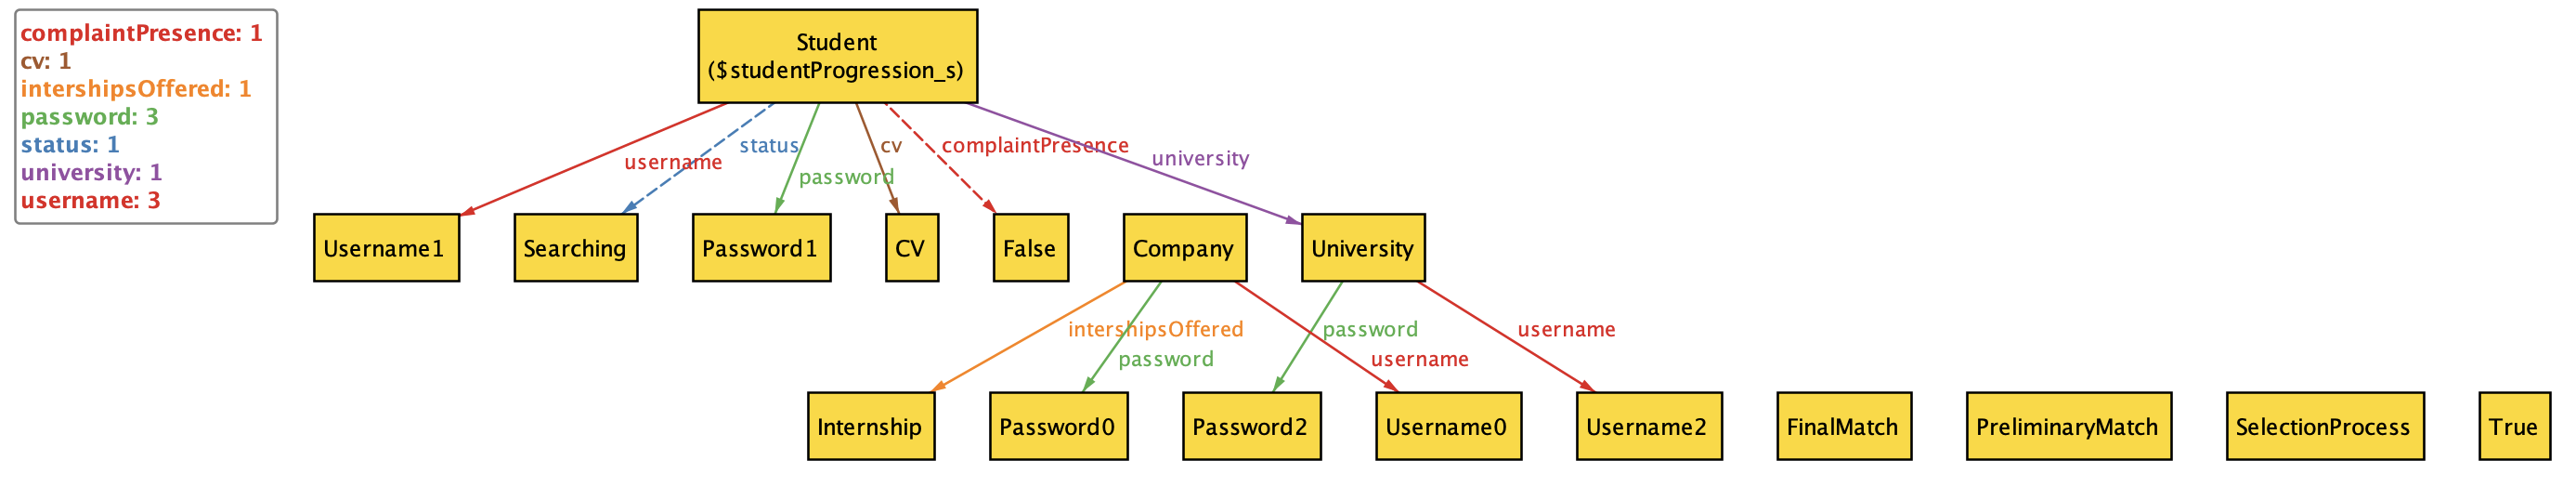
\includegraphics[width=\textwidth]{a1.png}

\subsubsection*{Instant 1: Initial State}
The system begins with a single \textbf{Student} in the \textbf{\textit{Searching}} status, actively looking for an internship. At this stage, the student's \texttt{complaintPresence} is set to \textbf{\texttt{False}}, indicating no complaints have been filed. The \texttt{internship} field is \textbf{\texttt{none}}, aligning with the requirement that students in the \textbf{\textit{Searching}} status cannot have an internship assigned. This state is stable and represents the starting point of the student's progression.
\\
\hrule
\vspace{5mm}
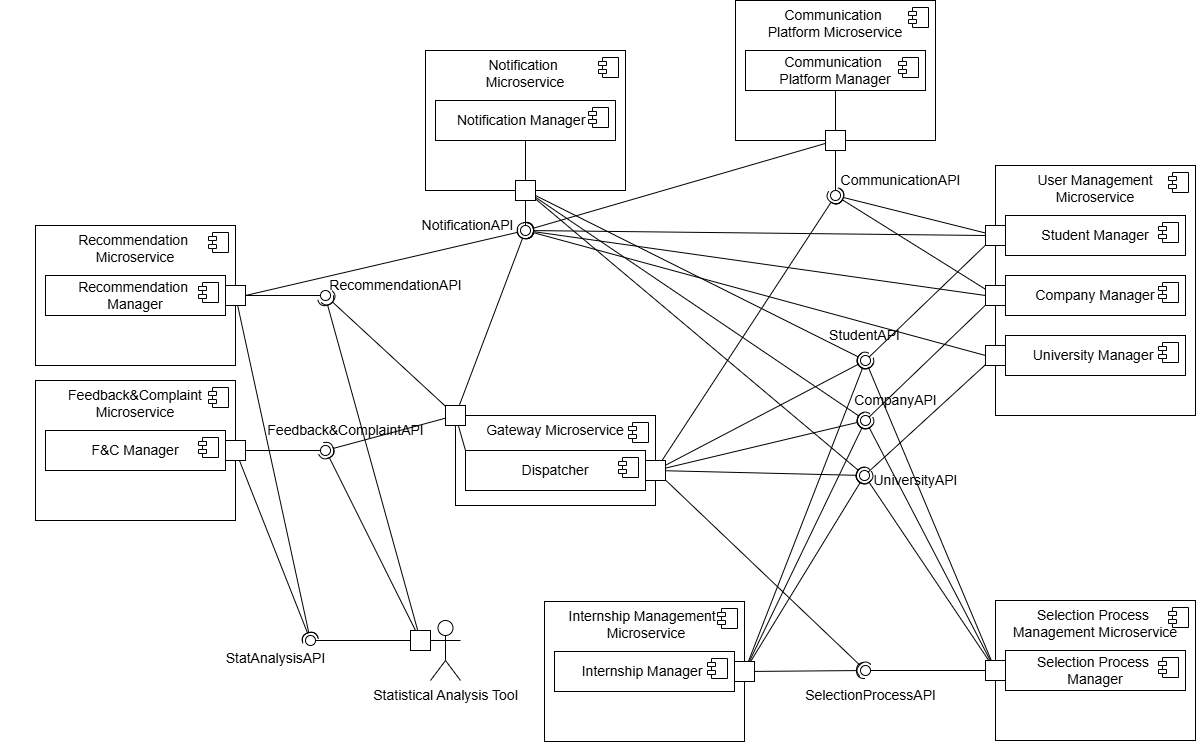
\includegraphics[width=\textwidth]{a2.png}

\subsubsection*{Instant 2: Preliminary Match}
The student transitions to the \textbf{\textit{PreliminaryMatch}} status, signifying the first significant step in their progression. The \texttt{internship} field is now associated with a specific internship offered by a company, demonstrating a tentative match between the student and the internship. The \texttt{complaintPresence} remains \textbf{\texttt{False}}, ensuring compliance with the fact that the student in this status does not have unresolved complaints. This evolution reflects the student's movement closer to securing an internship.
\\
\hrule
\vspace{5mm}
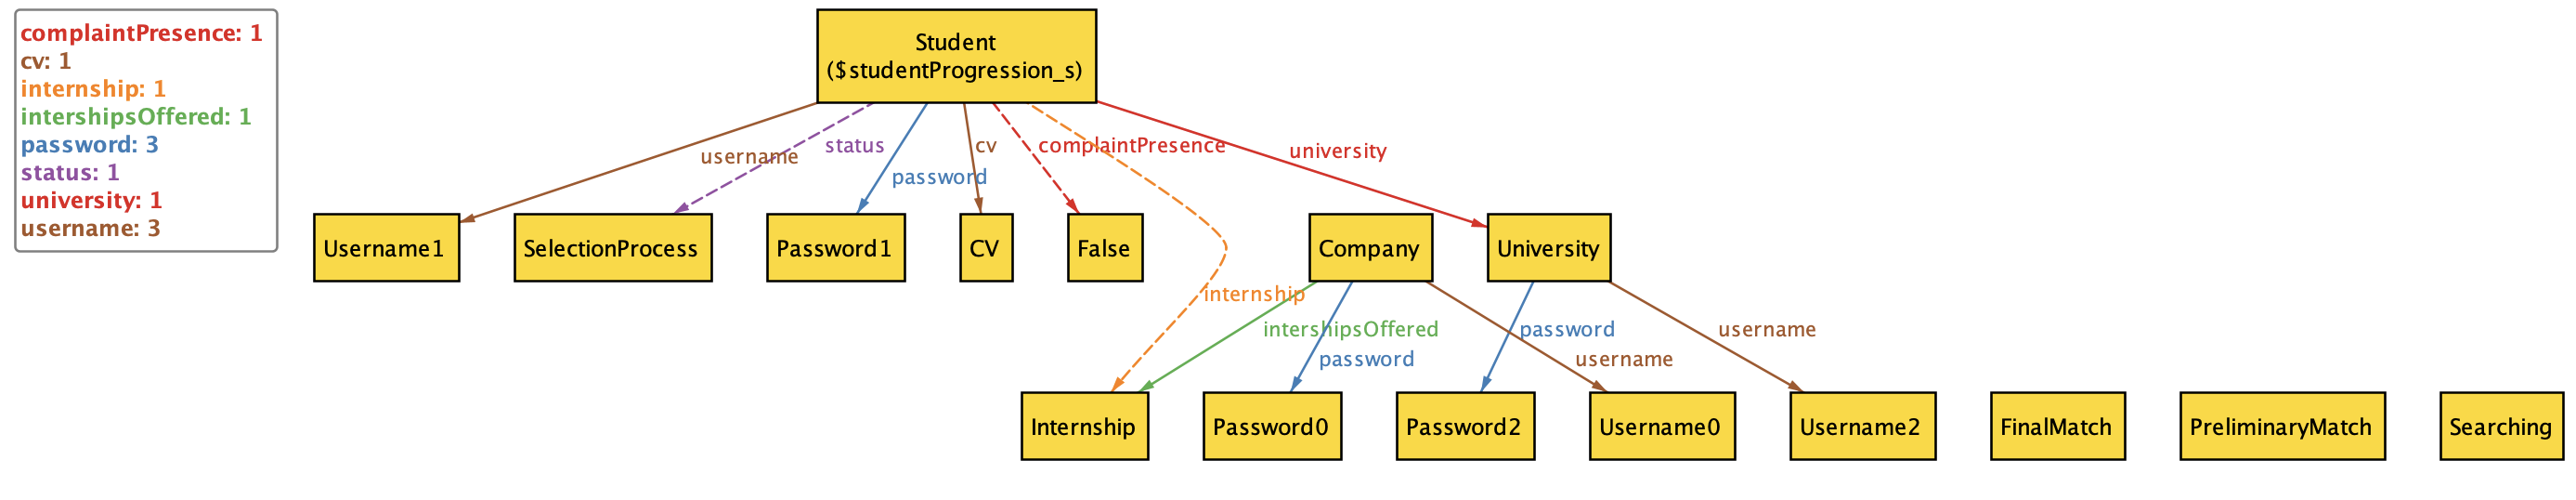
\includegraphics[width=\textwidth]{a3.png}

\subsubsection*{Instant 3: Selection Process}
In this instant, the student progresses further to the \textbf{\textit{SelectionProcess}} status. This transition signifies the student's entry into an evaluation phase for the assigned internship. Both the \texttt{internship} and \texttt{complaintPresence} fields remain unchanged, ensuring the continuity of their association with the preliminary match. This evolution highlights the system's adherence to the predefined progression hierarchy, advancing the student toward a possible final match.
\\
\hrule
\vspace{5mm}
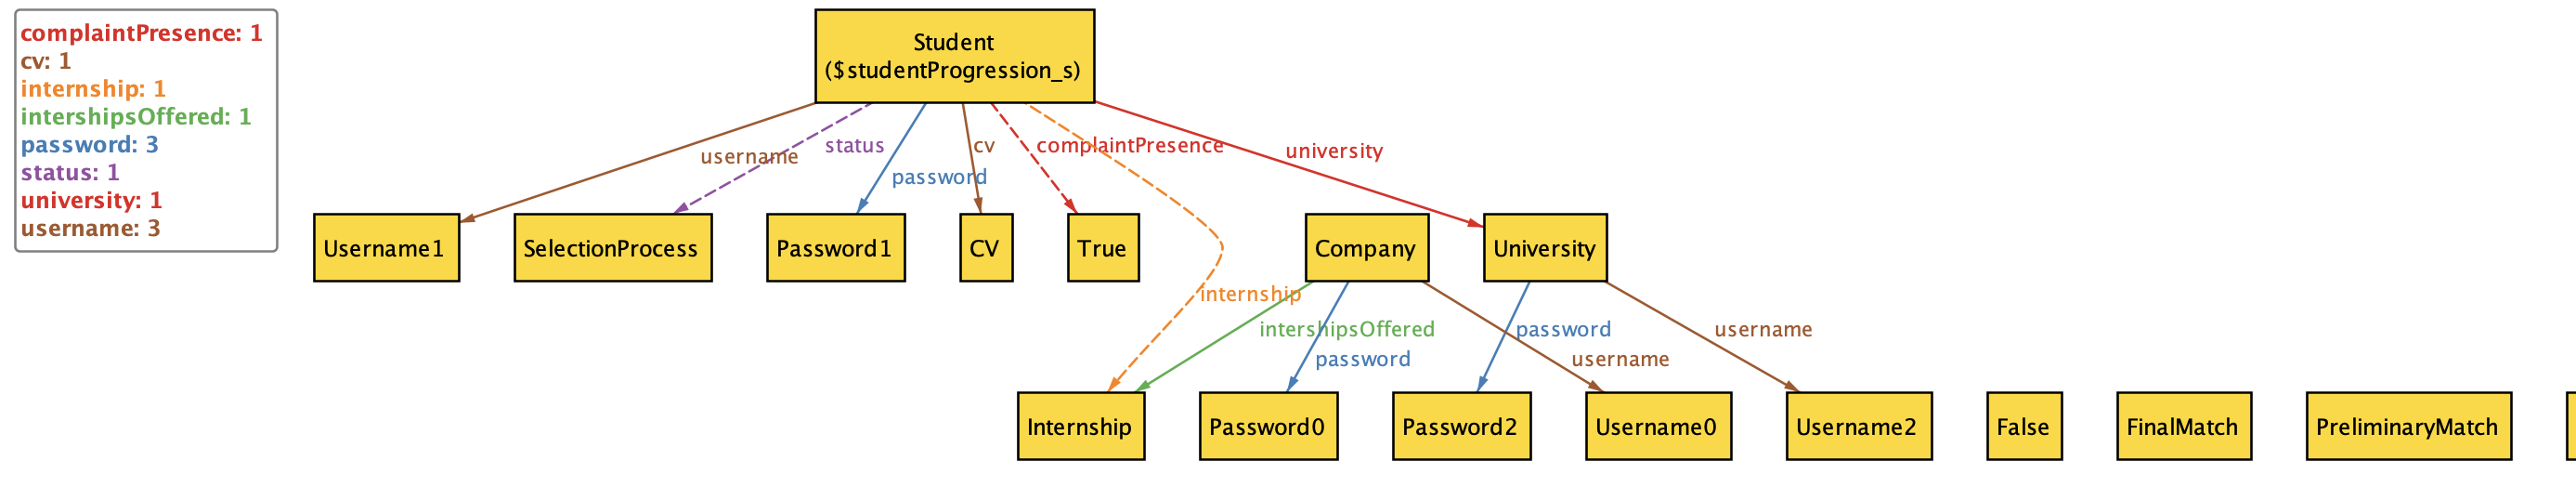
\includegraphics[width=\textwidth]{a4.png}

\subsubsection*{Instant 4: Complaint Registered}
A new development occurs where the \texttt{complaintPresence} changes from \textbf{\texttt{False}} to \textbf{\texttt{True}}. This indicates that the company or another entity has raised a concern or issue regarding the student. Despite this change, the \texttt{status} and \texttt{internship} fields remain unaffected, showing that the complaint is logged without disrupting the ongoing selection process. This state marks the introduction of external feedback into the student's progression.
\\
\hrule
\vspace{5mm}
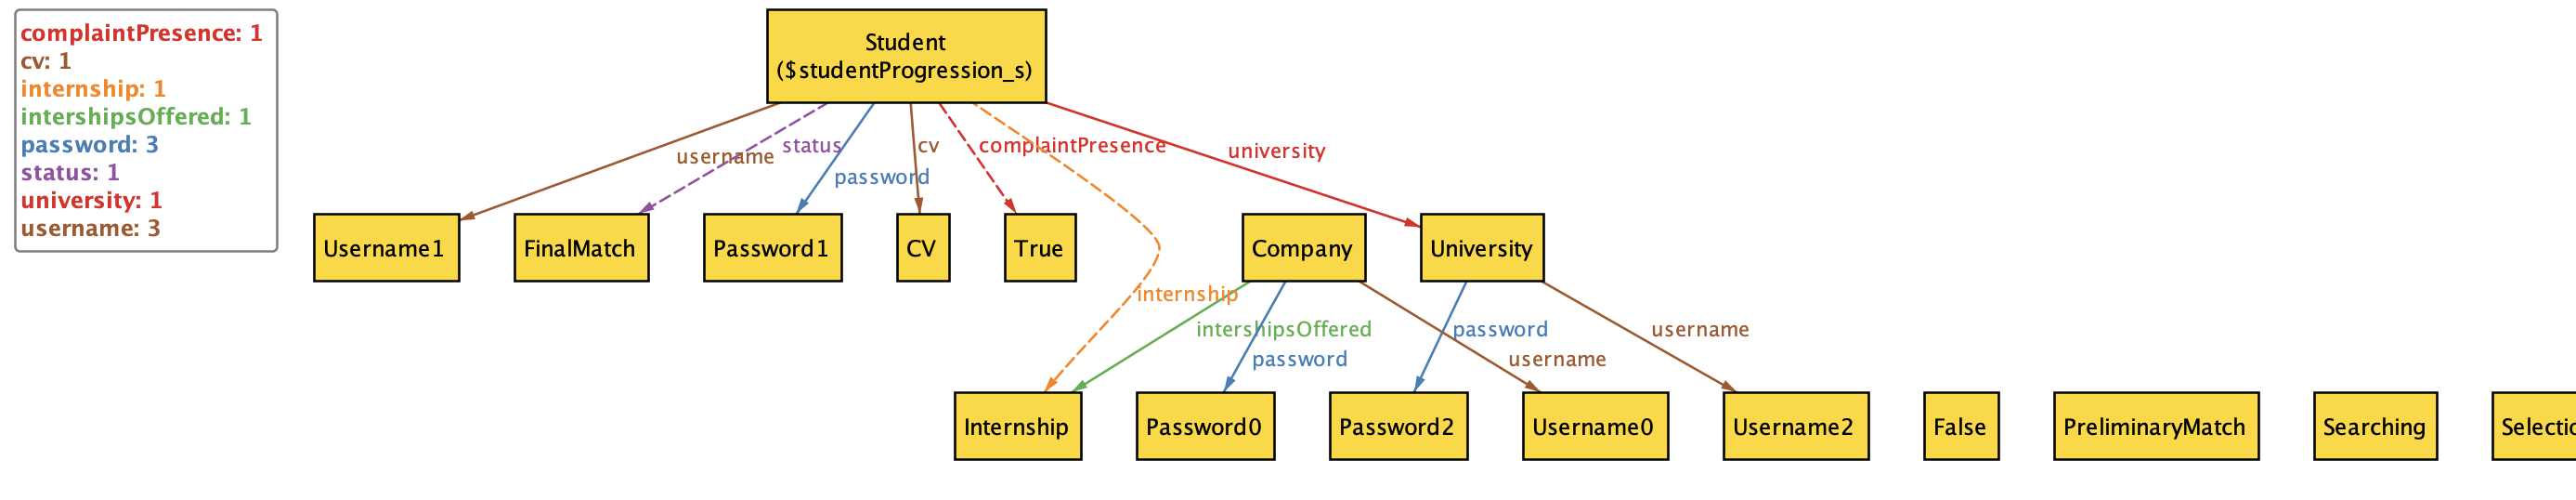
\includegraphics[width=\textwidth]{a5.png}

\subsubsection*{Instant 5: Final Match}
The student successfully advances to the \textbf{\textit{FinalMatch}} status, indicating they have secured the internship after completing the selection process. The \texttt{internship} association remains intact, reflecting their confirmed placement.
\\
\hrule
\vspace{5mm}
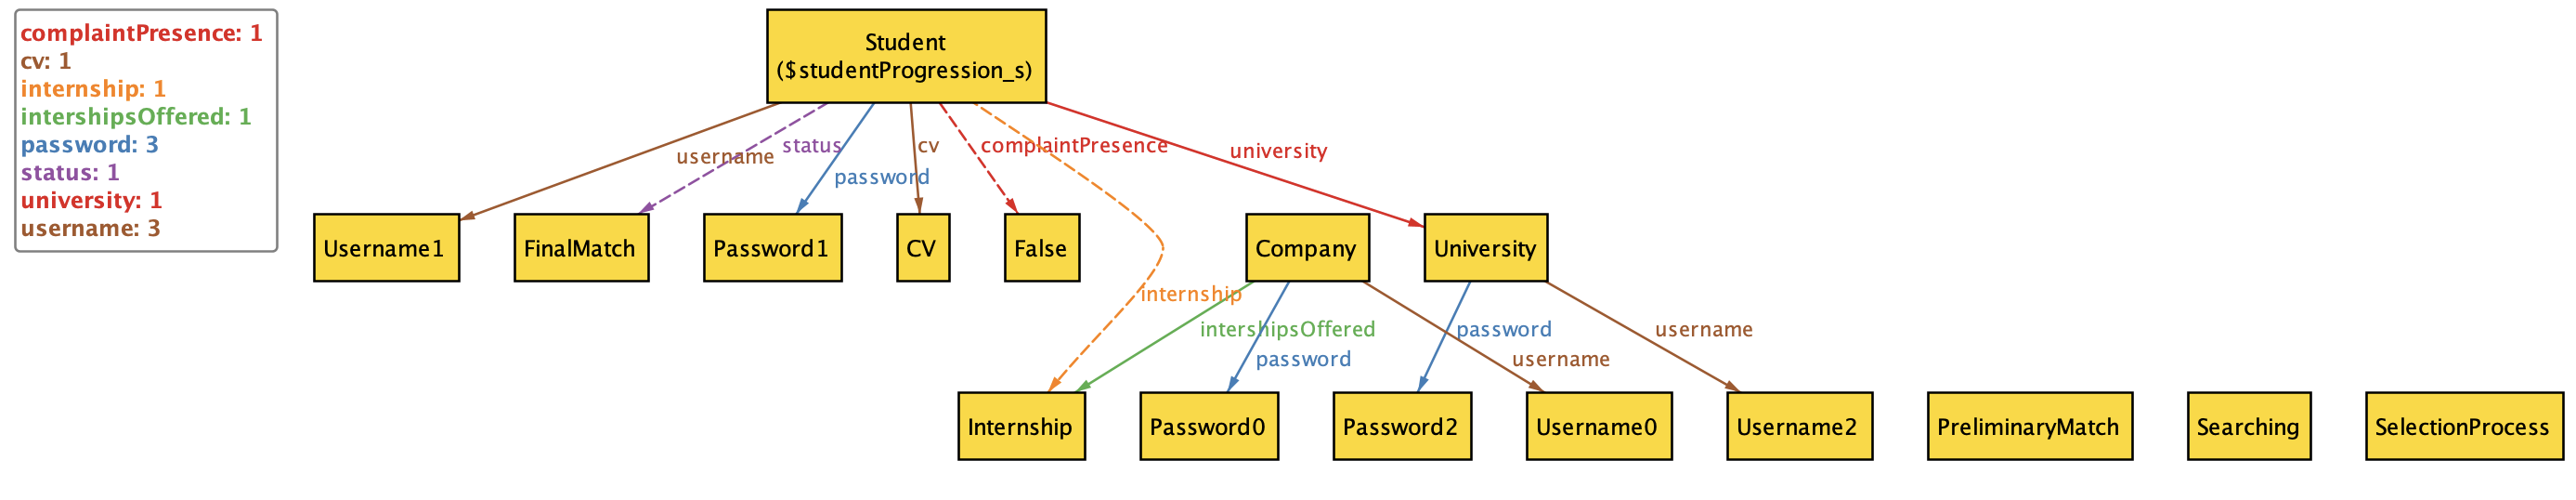
\includegraphics[width=\textwidth]{a6.png}

\subsubsection*{Instant 6: Complaint Removed}
The student remains in the \textbf{\textit{FinalMatch}} status, and their \texttt{internship} association is preserved. Importantly, the \texttt{complaintPresence} reverts to \textbf{\texttt{False}}, signifying resolution or removal of the previously registered complaint.
\\
\hrule
\vspace{5mm}
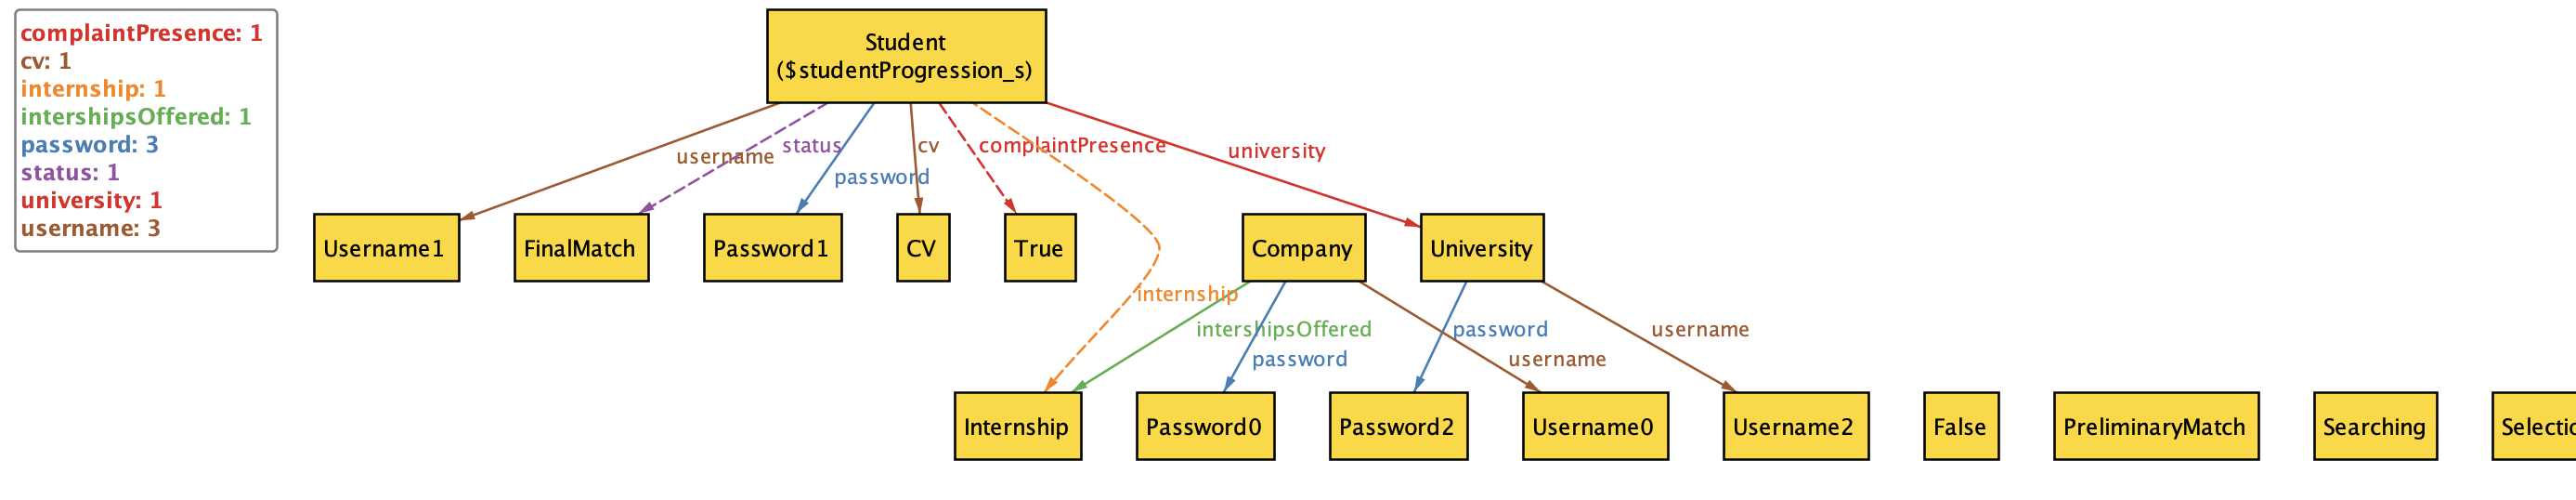
\includegraphics[width=\textwidth]{a7.png}

\subsubsection*{Instant 7: Return to Searching}
The student transitions back to the \textbf{\textit{Searching}} status, marking a reset in their progression. The \texttt{internship} field is set to \textbf{\texttt{none}}, and the \texttt{complaintPresence} reverts to \textbf{\texttt{False}}, demonstrating a clean slate for the student. This evolution likely represents the end of the internship or a termination event, initiated either by the student, the university, or another actor. This state brings the progression full circle, aligning with the cyclic nature of internship matching.

% //////////////////////////////
% ------------------------------
\subsection{Multiple Entities}
% ------------------------------
% //////////////////////////////

\vspace{5mm}
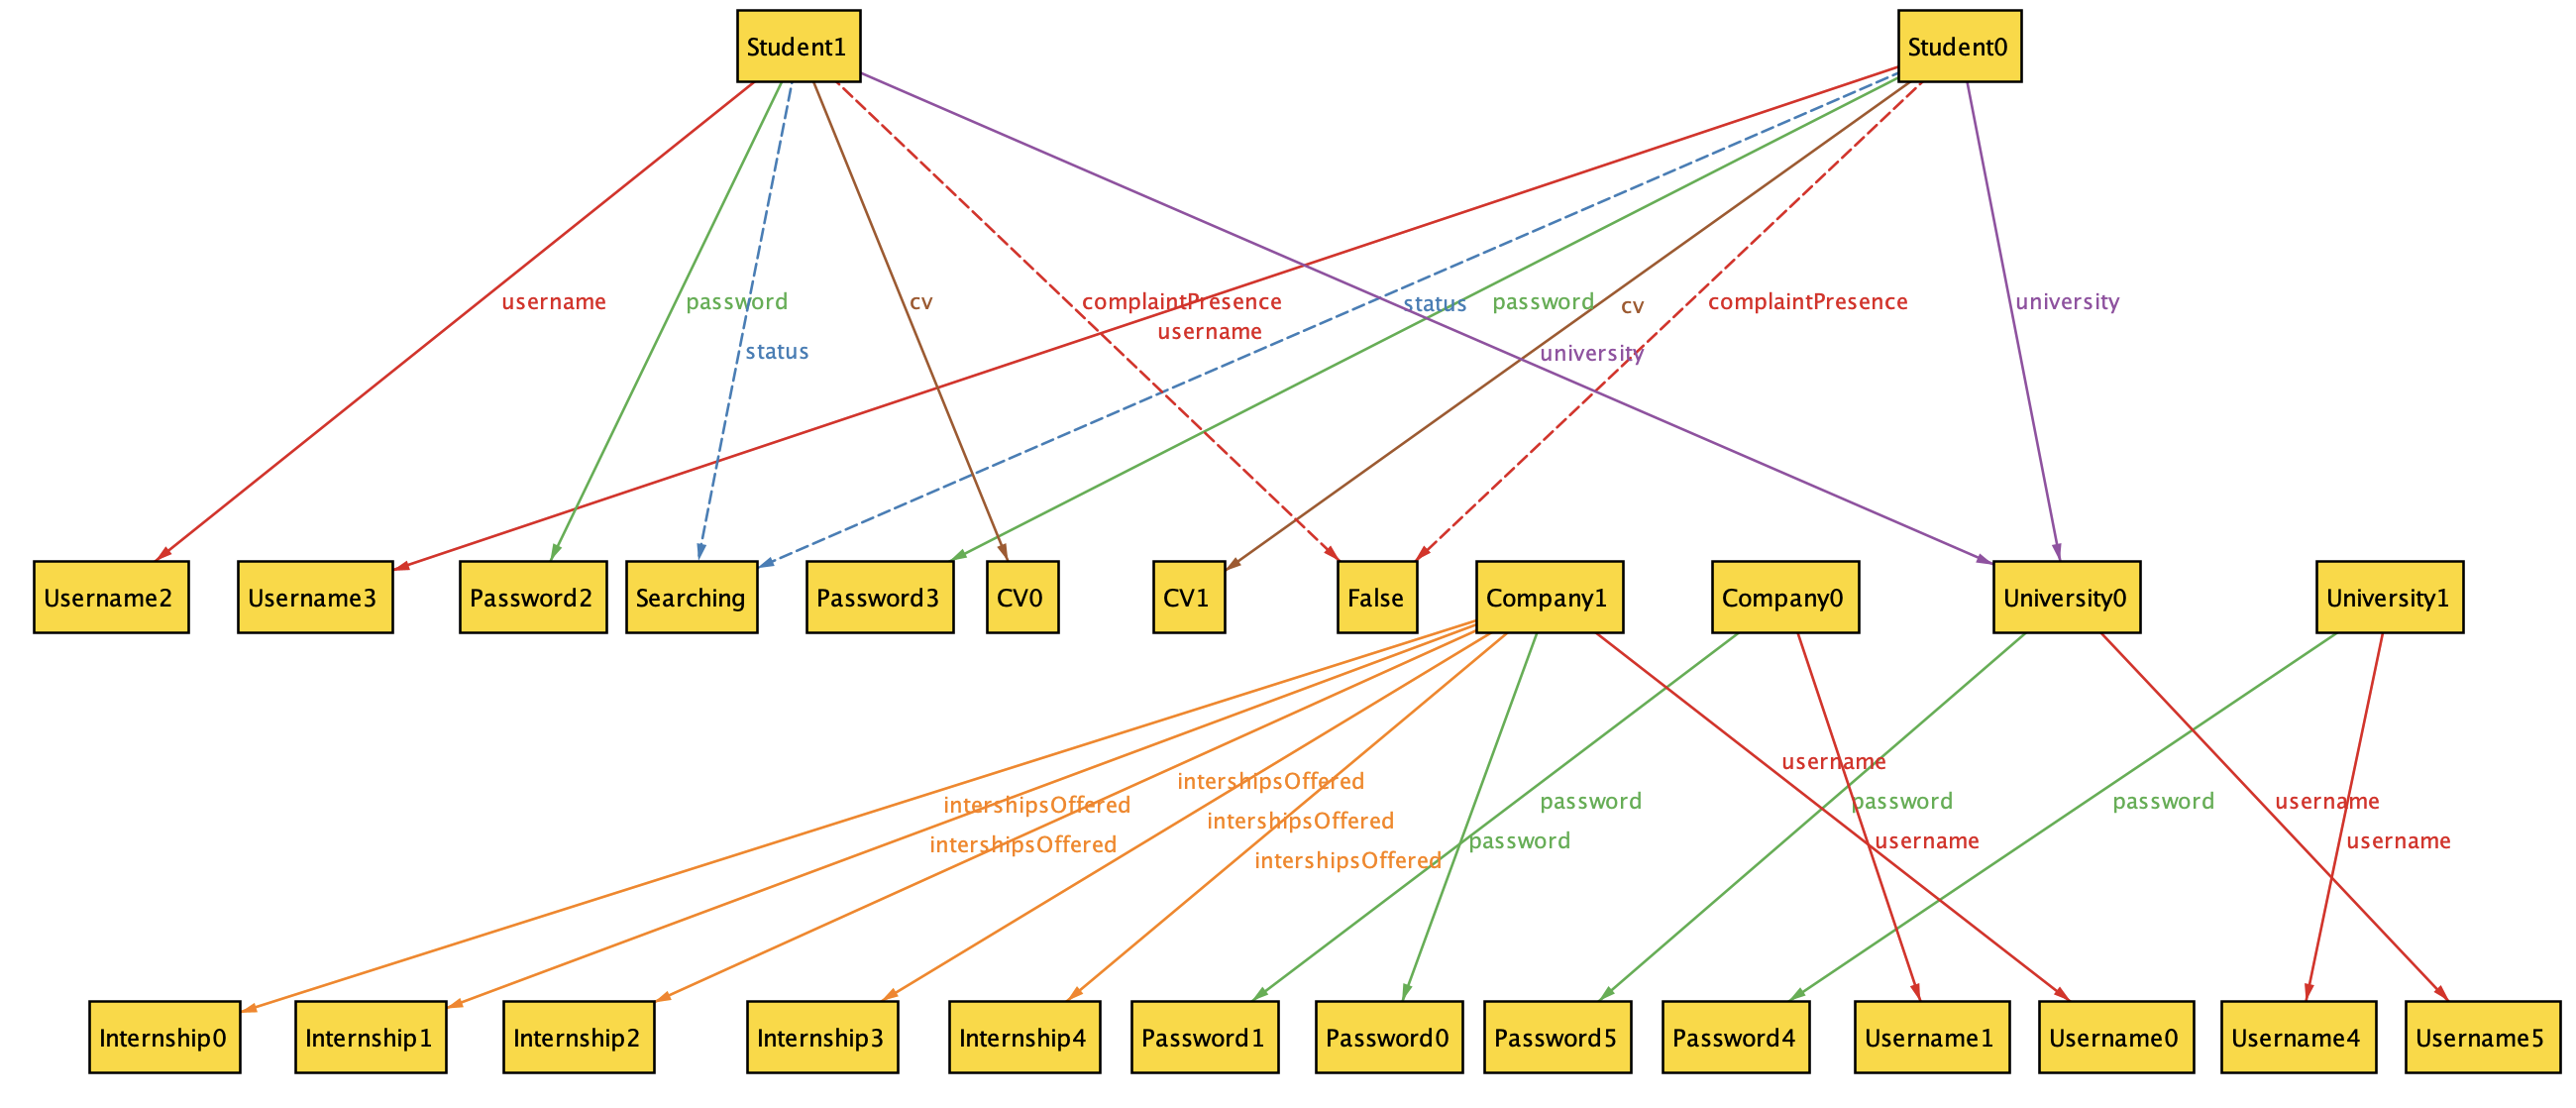
\includegraphics[width=\textwidth]{complex.png}

\subsubsection*{Complex State with Multiple Students} In this new, more complex world, we now observe two students within the system. Both students have distinct progressions, but they are at different stages of their internship journey. The first student remains in the \textbf{\textit{Searching}} status, while the second student has recently transitioned to the \textbf{\textit{PreliminaryMatch}} status, indicating that they have found a potential internship match. The \texttt{internship} fields for this last student is populated, reflecting his internship assignments. Importantly, the \texttt{complaintPresence} is \textbf{\texttt{False}} for both students, suggesting that no complaints are present at this moment. This screenshot highlights the diversity of student experiences within the system, with one student during matching process and the other still in the early stages of searching an internship. The presence of multiple students in different statuses shows the system's capacity to handle multiple entities and track their progress individually while maintaining the overall coherence of the internship matching process.